\documentclass[aspectratio=169,10pt]{beamer}

% ============================================================
%  Curso de Maestría — Métodos de Optimización
%  Introducción: el problema del sultán / de la secretaria
%  (parada óptima -- optimal stopping)
% ============================================================

\usepackage[utf8]{inputenc}
\usepackage[T1]{fontenc}
\usepackage{lmodern}
\usepackage[spanish]{babel}
\usepackage{amsmath,amssymb,amsthm}
\usepackage{graphicx}
\usepackage{booktabs}
\usepackage{xcolor}
\usepackage{listings}
\usepackage{tikz}

\graphicspath{{figs/}}

\usetheme{metropolis}
\metroset{block=fill, progressbar=frametitle, sectionpage=progressbar, numbering=fraction}

\definecolor{pygreen}{RGB}{0,128,0}
\definecolor{pyblue}{RGB}{0,0,180}
\definecolor{pygray}{RGB}{110,110,110}
\definecolor{codebg}{RGB}{245,245,245}

\lstdefinestyle{pythonstyle}{
  language=Python,
  backgroundcolor=\color{codebg},
  basicstyle=\ttfamily\scriptsize,
  keywordstyle=\color{pyblue}\bfseries,
  commentstyle=\color{pygreen}\itshape,
  stringstyle=\color{pygray},
  numbers=none,
  breaklines=true,
  showstringspaces=false,
  frame=single,
  rulecolor=\color{gray!40},
  xleftmargin=4pt,
  xrightmargin=4pt,
  aboveskip=6pt,
  belowskip=2pt,
}
\lstset{style=pythonstyle}

% --- notación abreviada ---
\newcommand{\R}{\mathbb{R}}
\newcommand{\grad}{\nabla}
\newcommand{\x}{\mathbf{x}}

\title{Métodos de Optimización}
\subtitle{Introducción: el problema del sultán (o de la secretaria)}
\author{[Nombre del profesor]}
\institute{Programa de Maestría, [Nombre de la universidad / programa]}
\date{Septiembre de 2026}

\begin{document}

% ---------------------------------------------------------------
\begin{frame}[plain]
  \maketitle
\end{frame}

\begin{frame}{Un tipo de búsqueda distinto a todo lo visto}
  Hasta ahora hemos buscado mínimos pudiendo \textbf{volver atrás}:
  reoptimizar, saltar de nuevo, mantener una población, comparar contra
  el mejor histórico. Hoy, para abrir el tema, un problema con una
  restricción brutal:
  \begin{alertblock}{La regla}
    Las opciones se presentan \textbf{una por una, en orden aleatorio}.
    Cada vez hay que decidir \textbf{en el momento}: aceptar o
    rechazar. \textbf{No se puede volver} a una que ya se rechazó, ni
    se sabe qué viene después.
  \end{alertblock}
  Esto se llama un problema de \textbf{parada óptima}
  (\emph{optimal stopping}) -- y tiene una solución sorprendentemente
  simple y elegante.
\end{frame}

\begin{frame}{El planteamiento formal}
  \begin{block}{}
    Hay $n$ candidatas, presentadas en orden aleatorio. Se puede
    comparar cada candidata nueva contra todas las anteriores (saber
    si es la mejor \emph{hasta ahora}), pero no se conoce su
    calidad absoluta ni cuántas faltan por venir. Tras ver una
    candidata hay que decidir de inmediato: quedarse con ella (fin
    del proceso) o descartarla (para siempre). Objetivo: maximizar la
    probabilidad de quedarse exactamente con \textbf{la mejor de las
    $n$}.
  \end{block}
  \small Este problema tiene muchos nombres según la historia con la
  que se cuenta: \emph{problema de la secretaria}, \emph{problema del
  matrimonio}, \emph{problema de la dote del sultán},
  \emph{problema del pretendiente quisquilloso}, \emph{juego del
  googol}.
\end{frame}

% ==================================================================
\section{La historia (o las historias)}
% ==================================================================

\begin{frame}{La dote del sultán}
  \begin{block}{El cuento}
    Un sultán permite que un plebeyo se case con una de sus cien
    hijas, con una condición: las hijas se presentan una por una, cada
    una revela su dote, y el pretendiente debe aceptar o rechazar en
    el acto. Solo puede casarse con la de \textbf{mayor dote de
    todas} -- si deja pasar a la mejor, no hay vuelta atrás.
  \end{block}
  \begin{alertblock}{La pregunta}
    ¿Qué estrategia maximiza la probabilidad de que el pretendiente
    termine casado con la hija de mayor dote?
  \end{alertblock}
\end{frame}

\begin{frame}{¿Un sultán legendario inventó esto? No exactamente}
  A pesar del disfraz narrativo, \textbf{no es un mito antiguo} -- es
  un acertijo matemático de mediados del siglo XX:
  \begin{itemize}
    \item \textbf{1949}: Merrill Flood lo plantea en una conferencia
      como el \emph{problema de la prometida}.
    \item Circula informalmente en los años 50 (incluyendo una prueba
      en una carta de Flood de 1958).
    \item \textbf{Febrero de 1960}: primera publicación, en la columna
      de Martin Gardner en \emph{Scientific American}. Gardner lo
      conoció por John Fox y Gerald Marnie (\emph{el juego del googol});
      Leo Moser aportó el análisis matemático correcto.
    \item Antecedente más antiguo: Arthur Cayley planteó un problema
      similar en \textbf{1875}.
  \end{itemize}
  El \emph{sultán} es solo el disfraz más memorable de un problema mucho
  más reciente.
\end{frame}

\begin{frame}{La historia real: Johannes Kepler}
  \begin{block}{Un caso genuino, no un cuento}
    El astrónomo \textbf{Johannes Kepler} sí enfrentó este problema en
    la vida real. Entre \textbf{1611 y 1613}, tras enviudar, dedicó
    casi dos años a buscar nueva esposa: entrevistó (en la práctica)
    a \textbf{11 candidatas} sucesivas antes de decidirse por una.
  \end{block}
  Kepler documentó por escrito su razonamiento sobre por qué rechazó a
  varias candidatas prometedoras al principio -- sin saberlo, estaba
  aplicando la misma lógica que formalizaría la matemática 300 años
  después: \emph{no decidirse demasiado pronto, pero tampoco esperar
  demasiado.}
\end{frame}

% ==================================================================
\section{La solución: la regla del 1/e}
% ==================================================================

\begin{frame}{La estrategia óptima}
  \begin{block}{La regla del 37\%}
    Fijar un umbral $k$. \textbf{Rechazar automáticamente} a las
    primeras $k$ candidatas -- solo sirven para calibrar qué tan buena
    es \emph{buena}. Después, \textbf{aceptar a la primera} candidata que
    sea mejor que \textbf{todas} las anteriores (un \emph{récord}).
  \end{block}
  \begin{alertblock}{El resultado}
    El $k$ óptimo satisface $k/n \to 1/e \approx 0.368$. Para $n=100$:
    rechazar a las primeras $\approx 37$ y quedarse con la primera que
    rompa el récord después. La probabilidad de terminar con la
    \textbf{mejor de todas} converge a $1/e\approx 36.8\%$ --
    \textbf{sin importar} si $n=100$ o $n=100$ millones.
  \end{alertblock}
\end{frame}

\begin{frame}{¿De dónde sale el $1/e$?}
  Sea $P(k)$ la probabilidad de éxito rechazando las primeras $k$. Si
  la mejor candidata de todas está en la posición $i$, se le atrapa
  \emph{si y solo si} la mejor de las primeras $i-1$ está entre las
  $k$ rechazadas (si no, algo entre $k$ e $i-1$ ya habría sido
  aceptado antes de llegar a $i$). Sumando sobre todas las posiciones
  $i$ posibles:
  \[
    P(k) = \frac{k}{n}\sum_{i=k+1}^{n}\frac{1}{i-1}
  \]
  Con $x=k/n$ y $n\to\infty$, la suma se aproxima a $-\ln x$, así que
  \[
    P(x) \approx -x\ln x .
  \]
  Maximizando: $\dfrac{d}{dx}(-x\ln x) = -\ln x - 1 = 0
  \;\Rightarrow\; x=\dfrac{1}{e}$, y el máximo vale
  $P\!\left(\tfrac1e\right) = \dfrac1e$.
\end{frame}

% ==================================================================
\section{Verificación por simulación}
% ==================================================================

\begin{frame}[fragile]{Verificación por Monte Carlo: código}
\begin{lstlisting}
def tasa_exito_simulada(k, n, trials, rng):
    perms = np.array([rng.permutation(n) + 1 for _ in range(trials)])
    mejor_visto = perms[:, :k].min(axis=1) if k > 0 else np.full(trials, np.inf)
    candidatas = perms[:, k:]
    es_record = candidatas < mejor_visto[:, None]      # mejor que TODO lo anterior
    hubo_eleccion = es_record.any(axis=1)
    idx_primero = np.argmax(es_record, axis=1)          # primer record
    elegida = candidatas[np.arange(trials), idx_primero]
    exito = hubo_eleccion & (elegida == 1)               # 1 = rango de la mejor
    return exito.mean()

def tasa_exito_teorica(k, n):
    if k == 0: return 1.0 / n
    return (k/n) * sum(1.0/(i-1) for i in range(k+1, n+1))
\end{lstlisting}
  Script completo: \texttt{scripts/01\_regla\_1e\_simulacion.py}
\end{frame}

\begin{frame}{Verificación por Monte Carlo: resultado}
  \begin{center}
    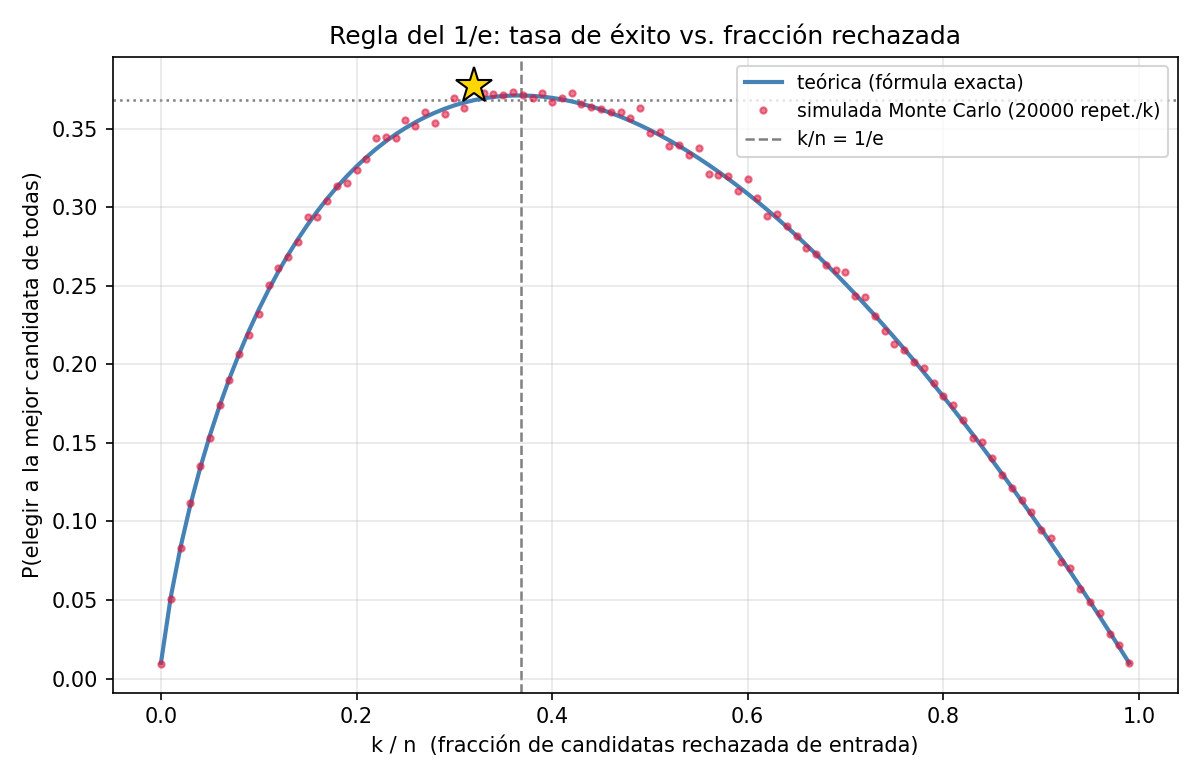
\includegraphics[height=6.3cm,keepaspectratio]{fig_secretaria_1e.png}
  \end{center}
\end{frame}

\begin{frame}{Lo que muestra la simulación}
  \begin{itemize}
    \item $n=100$ candidatas, 20{,}000 repeticiones Monte Carlo por
      cada valor de $k$: la curva simulada (puntos) coincide casi
      exactamente con la fórmula teórica exacta (línea).
    \item El óptimo empírico cae muy cerca de $k/n=1/e\approx0.368$,
      con tasa de éxito $\approx 37\%$ -- tal como predice la teoría.
    \item \textbf{La curva es muy plana cerca del óptimo}: rechazar
      30, 35 o 40 candidatas (en vez de exactamente 37) apenas cambia
      la tasa de éxito. La regla del $1/e$ no exige precisión
      quirúrgica para ser útil.
  \end{itemize}
\end{frame}

% ==================================================================
\section{Conexión con el curso}
% ==================================================================

\begin{frame}{¿Por qué empezar (o hacer una pausa) aquí?}
  \begin{block}{El contraste es el punto}
    Todos los métodos de las Clases 2 y 3 (grid search, random walk,
    Nelder--Mead, basin hopping, simulated annealing, algoritmos
    genéticos, PSO) permiten \textbf{revisar, reoptimizar o mantener
    varias soluciones en paralelo}. El problema del sultán es la
    versión más extrema y más simple del caso opuesto: decisiones
    \textbf{irreversibles}, \textbf{una sola pasada}, información
    \textbf{online} (nunca se ve el futuro).
  \end{block}
  \begin{exampleblock}{Familia más amplia}
    Esta es la puerta de entrada a la teoría de \textbf{parada
    óptima} y a los \textbf{algoritmos online} -- relevantes en
    asignación de recursos en tiempo real, búsqueda de empleo/vivienda,
    contratación, y trading, entre muchos otros.
  \end{exampleblock}
\end{frame}

\begin{frame}{Referencias}
  \footnotesize
  \begin{itemize}
    \item M. Flood. Correspondencia y notas sobre el \emph{problema de la
      prometida}, 1949--1958 (no publicado formalmente).
    \item M. Gardner. \emph{Mathematical Games}. Scientific American,
      febrero de 1960.
    \item A. Cayley. \emph{Mathematical Questions with Their Solutions}.
      Educational Times, 1875.
    \item T. Ferguson. \emph{Who Solved the Secretary Problem?}
      Statistical Science, 4(3), 1989. (Historia completa del
      problema, incluye el caso de Kepler.)
    \item P. Freeman. \emph{The Secretary Problem and its Extensions: A
      Review}. International Statistical Review, 51(2), 1983.
    \item Wikipedia: \emph{Secretary problem}; \emph{Sultan's Dowry}.
  \end{itemize}
\end{frame}

\begin{frame}[standout]
  ¿Preguntas?
\end{frame}

\end{document}
